\documentclass{article}
\usepackage{tikz}
\usetikzlibrary{snakes}
\usetikzlibrary{calc,decorations.markings}
\usepackage[compat=1.1.0]{tikz-feynman}
\usepackage{pgfplots}
\usepackage[colorinlistoftodos]{todonotes}

\begin{document}

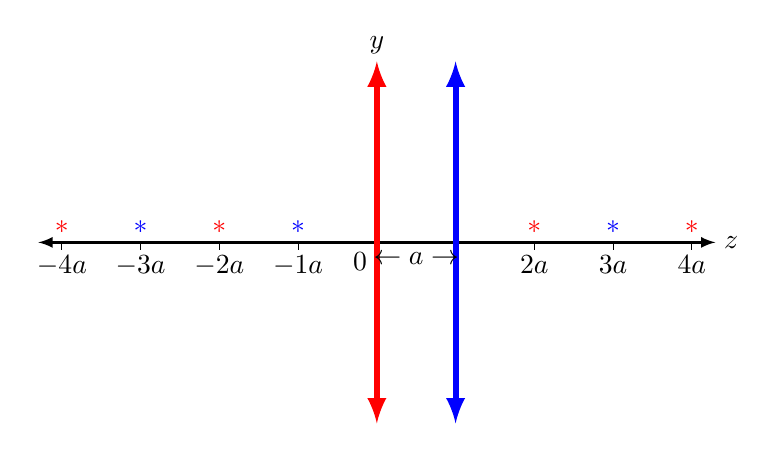
\begin{tikzpicture} 
\def \minx {-4}
\def \maxx {4}
\def \miny {-2}
\def \maxy {2}


\draw[thick, latex-latex] (\minx-0.3,0)--(\maxx+0.3,0);
\draw[red,line width=0.75mm,latex-latex] (0,\miny-0.3)--(0,\maxy+0.3);
\draw[blue,line width=0.75mm,latex-latex] (1,\miny-0.3)--(1,\maxy+0.3);
\node at (\maxx+0.5,0) {$z$};
\node at (0,\maxy+0.5) {$y$};

\foreach \x in {\minx,...,-1}{
    \draw (\x,0)--(\x,-0.1);
    \node[below,black] at (\x,-0.05) {$\x a$};
}
\foreach \x in {2,...,\maxx}{
    \draw (\x,0)--(\x,-0.1);
    \node[below,black] at (\x,-0.05) {$\x a$};
}
\node[below left,black] at (0,0) {$0$};
\node[below ,black] at (0.5,0.0) {$\leftarrow a \rightarrow$}; 

\node[red] at (2,0.2) {$\ast$};
\node[red] at (4,0.2) {$\ast$};
\node[red] at (-2,0.2) {$\ast$};
\node[red] at (-4,0.2) {$\ast$};

\node[blue] at (3,0.2) {$\ast$};
\node[blue] at (-1,0.2) {$\ast$};
\node[blue] at (-3,0.2) {$\ast$};

\end{tikzpicture}

\end{document}